% !Mode:: "TeX:UTF-8"


\chapter{广义同步数据流图转化为任务的有向无环图}
% ICS 算法
上一章得到了包含时间约束的 GSDF 图,下面需要生成对应的 DAG 图。通过 \ref{SDF-intro} 节中介绍的\cite{SDF1987}中的S类算法可以将GSDF转化为对应的DAG,但由于本文需要考虑通信问题,因此这个过程中也需要加入对数据的特殊处理。此外,虚拟结点在转化过程中也有其特殊含义。

\section{求解拓扑矩阵}
% 简述 从 GSDF 到 DAG 的过程
% 最小整数解中 q_0 的意义表示最小周期的长度

用 \ref{SDF-intro} 节中提到的方法可以得到 GSDF 图对应的拓扑矩阵 $\Gamma$。 为方便起见,假定 $\Gamma$ 的列的下标分别为 $0, 1, 2, \dots, n$,其中第 0 列对应的是虚拟结点,而 $1, \dots, n$ 列分别对应任务结点 $t_1, t_2, \dots, t_n$。 根据 \eqref{basic-eq-matrix} 式可以求得 $\Gamma$ 零向量空间的最小整数解为 $\textbf{q}$,其中虚拟结点所对应的 $\textbf{q}_0$ 即表示在一个最小周期中,虚拟任务将会被运行几次。根据 \ref{SDF-time-constraint} 节对虚拟结点所做的两点假定,可知虚拟结点在周期内一定串行且无间隔的连续执行,而每个虚拟任务的执行时间是单位时间,因此即有推论 $\textbf{q}_0$ 的值即为一个最小调度周期的长度。


\section{周期内结点间的数据传输}
\label{DAG-innerp}

SDF 图中任务之间数据吞吐速率可以是不同的,例如任务 A 与 B 之间,每次 A 执行产生 3 个数据,而每次 B 执行仅消耗 2 个数据,造成A 每次产生的数据需要分别传送给DAG图中B的两次不同的执行结点,这样才能够正确处理A、B 任务多次执行之间的消息传递。另外,在两个调度周期交界处,前一周期的任务结点也需要向后一周期的任务结点发送数据,且需要在前一周期结束前传输完毕,以使第二周期的任务在周期开始时能够回到与前一周期相同的状态,周期性调度才能够继续下去,因此也需要解决周期之间任务结点的数据传输问题。下面分别讨论。


本节讨论一般情况下周期内结点间数据传输的处理方式。现有任务$t_i$与$t_j$ 之间存在数据依赖关系,如图\ref{DLS-fig-gendep}所示,每次$t_i$ 执行产生 $p_{ij}$ 个数据,而每次 $t_j$ 执行消耗 $c_{ij}$ 个数据,初始时 $t_i$到$t_j$ 的 Delay 为 $D_{ij}$。

\begin{figure}[!hbt]
  \centering
  % Requires \usepackage{graphicx}
  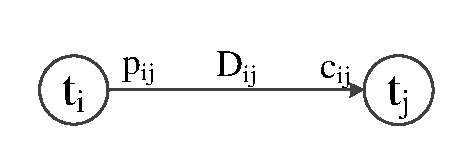
\includegraphics[height=8ex]{figure/DLS-gendep.pdf}\\
  \caption{SDF中$t_j$到$t_j$的一般依赖关系}\label{DLS-fig-gendep}
\end{figure}

需要解决的问题是求出$t_j$的第k次执行结点需要的数据分别来自$t_i$任务哪几次的运行结点,并求出分别需要的数据量是多少。从 \eqref{basic-eq-d} 式可以求得 $t_j$ 的第 k 次执行需要来自 $t_i$ 多少次执行的数据,但无法具体求出分别需要传输的数据量大小。为解决此问题,考察从 $t_i$ 到 $t_j$ 的数据量的对应关系,如图 \ref{DAG-fig-innerp-data} 所示。%如图所示。。。两行 分别表示产出 和 输入数据的对比图

\begin{figure}[!hbt]
  \centering
  % Requires \usepackage{graphicx}
  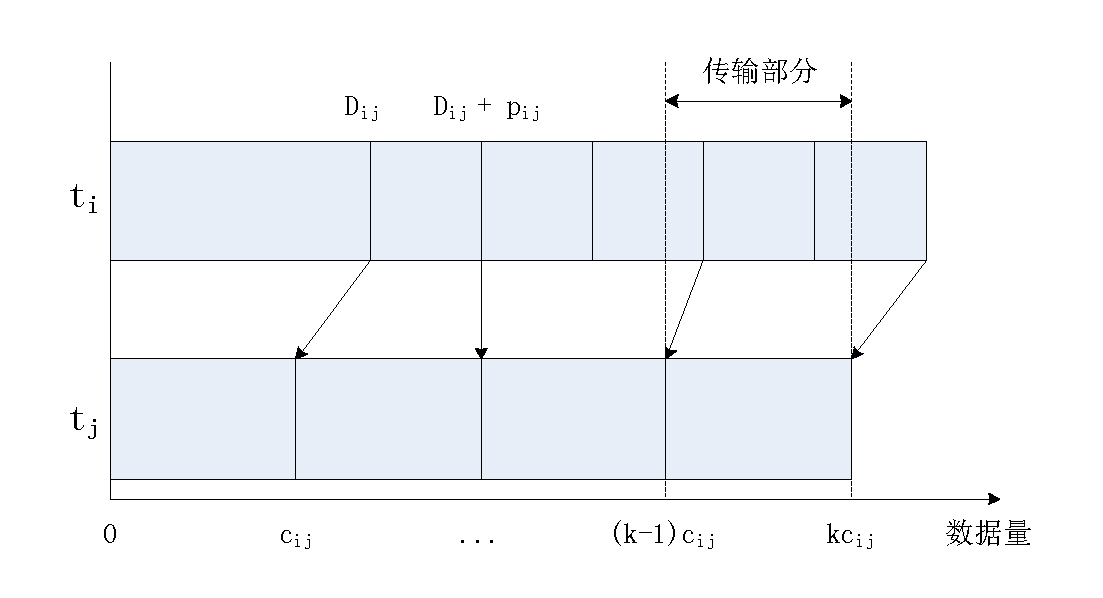
\includegraphics[height=30ex]{figure/DAG-innerp-data.pdf}\\
  \caption{DAG中$t_j$第k次运行与$t_i$的数据对应关系}\label{DAG-fig-innerp-data}
\end{figure}

任务 $t_j$ 的前k次执行共需数据量为
\begin{equation}
  \textnormal{Req}_{j}[k]=kc_{ij}
\end{equation}
前(k-1)次执行共需数据量为
\begin{equation}
  \textnormal{Req}_{j}[k-1]=(k-1)c_{ij}
\end{equation}
因此 $t_j$ 的第k次执行需要从 $(k-1)c_{ij}$ 到 $kc_{ij}$ 部分数据,如图 \ref{DAG-fig-innerp-data} 中虚线部分所示。下面来求这些数据与 $t_i$ 对应运行次数之间的数据关系,从图中可以看出,这部分数据来自 $t_i$ 与 $t_j$ 之间的 Delay 以及 $t_i$ 运行所产生的数据,即有
\begin{equation}\label{DAG-eq-innerp-eq1}
  D_{ij}+w_1p_{ij}+r_1=(k-1)c_{ij}
\end{equation}
和
\begin{equation}\label{DAG-eq-innerp-eq2}
  D_{ij}+w_2p_{ij}+r_2=kc_{ij}
\end{equation}
两式成立。其中 $r_1,r_2$ 表示边界情况时 $t_i$ 分别有部分数据需要传给不同的 $t_j$ 结点,$r_1,r_2$ 均为整数,且 $r_1\in[0,p_{ij})$ 而 $r_2\in[1,p_{ij}]$。
根据 \eqref{DAG-eq-innerp-eq1} 和 \eqref{DAG-eq-innerp-eq2} 式,以及以上对 $r_1,r_2$ 的约束可以解得
%\begin{equation*}
%  w_1=\left\lceil\frac{(k-1)c_{ij}-D_{ij}}{p_{ij}}\right\rceil
%\end{equation*}
%\begin{equation*}
%  r_1=(k-1)c_{ij}-D_{ij}-w_1p_{ij}
%\end{equation*}
%\begin{equation*}
%  w_2=\left\lceil\frac{kc_{ij}-D_{ij}-1}{p_{ij}}\right\rceil
%\end{equation*}
%\begin{equation*}
%  r_2=kc_{ij}-D_{ij}-w_2p_{ij}
%\end{equation*}
\begin{align}
  \label{DAG-eq-innerp-solve}
  w_1&=\left\lfloor\frac{(k-1)c_{ij}-D_{ij}}{p_{ij}}\right\rfloor\\
%  \label{DAG-eq-innerp-solve-2}
  r_1&=(k-1)c_{ij}-D_{ij}-w_1p_{ij}\\
%  \label{DAG-eq-innerp-solve-3}
  w_2&=\left\lfloor\frac{kc_{ij}-D_{ij}-1}{p_{ij}}\right\rfloor\\
  \label{DAG-eq-innerp-solve-ed}
  r_2&=kc_{ij}-D_{ij}-w_2p_{ij}
\end{align}

由以上四式可知,在边界条件下$t_i$的第$w_1$ 次运行需要传给$t_j$的第k次运行$p_{ij}-r_1$ 的数据量,而$t_i$的第$w_2$次运行需要传给$t_j$的第k次运行$r_2$的数据量。在边界条件中间的部分,每次 $t_i$ 运行产生的全部 $p_{ij}$ 数据都需要传给 $t_j$ 的第 k 次运行。当然,以上 $w_1$ 与 $w_2$ 也可能是相等的值,此时 $t_i$ 运行一次产生的数据量已大于 $t_j$ 的需求了,或者 $w_1<0$ 表示 $t_j[k]$ 结点有部分数据来自于 Delay 部分,这是下节要讨论的周期间数据传输的内容。

综上可知,$t_j$ 第 k 次运行的结点所需总数据满足以下关系:
\begin{equation}
  c_{ij}=(p_{ij}-r_1)+(w_2-w_1-1)p_{ij}+r_2
\end{equation}

根据以上所述内容,可以描述求出 $t_j[k]$ 结点依赖的周期内$t_i$结点数据传输量的过程如算法\ref{algo-DAG-innerp}所述。% 以后改为算法环境
\begin{algorithm}
  \caption{计算周期内结点间数据传输量}
  \label{algo-DAG-innerp}
  \KwIn{GSDF 图}
  \KwOut{DAG 中周期内结点间数据传输量}
  由\eqref{DAG-eq-innerp-solve}-\eqref{DAG-eq-innerp-solve-ed}四式求得 $w_1$、$r_1$、$w_2$ 和 $r_2$\;
  \uIf{$w_1==w_2$}{
      \If{$w_1 \geqslant 0$ AND $r_1 < r_2$}{
          添加从 $t_i[w_1+1]$ 到 $t_j[k]$ 结点的 $c_{ij}$ 大小的数据量\;
      }
  }
  \Else{
      \If{$w_1 \geqslant 0$}{
          添加从 $t_i[w_1+1]$ 到 $t_j[k]$ 结点的 $p_{ij}-r_1$ 大小的数据量\;
      }
      \For{$v=w_1+2$ TO $w_2$}{
          添加从 $t_i[v]$ 到 $t_j[k]$ 结点的 $p_{ij}$ 大小的数据量\;
      }
      \If{$w_2 \geqslant 0$}{
          添加从 $t_i[w_2+1]$ 到 $t_j[k]$ 结点的 $r_2$ 大小的数据量\;
      }
  }
\end{algorithm}

%\begin{Verbatim}[numbers=left,frame=single,xleftmargin=50pt,commandchars=\\\{\}]
%由上述四式求得 w1、r1、w2 和 r2。
%IF w1==w2 THEN
%    IF w1 >= 0 AND r1 < r2 THEN
%        添加从 ti[w1+1] 到 tj[k] 结点的 cij 大小数据量
%    END IF
%ELSE
%    IF w1 >= 0 THEN
%        添加从 ti[w1+1] 到 tj[k] 结点的 pij-r1 大小数据量
%    END IF
%    FOR v = w1 + 2 TO w2 DO
%        添加从 ti[v] 到 tj[k] 结点的 pij 大小数据量
%    END FOR
%    IF w2 >= 0 THEN
%        添加从 ti[w2+1] 到 tj[k] 结点的 r2 大小数据量
%    END IF
%END IF
%\end{Verbatim}

以上算法可加入 \cite{SDF1987} 所述的S 类算法过程中,在构造 DAG 的同时即可得到周期内结点间的具体数据传输量。在本章后面的小节中将给出一个包含了周期内数据传输以及周期间数据传输部分的改进的S 类算法,即 Imporved Class S Algorithm (ICS 算法)。


%\emph{TODO}: 给出周期内结点间数据传输的计算方法

\section{周期间结点间的数据传输}
\label{DAG-interp}

由于每个任务都需要将执行所产生的数据全部传输完毕才能保证下周期开始时系统回到相同的初始态,因此如果某个结点产生的数据向同周期内其他结点发送后仍留有剩余,那么该结点一定与下一周期内的任务存在数据传输关系,需要传输的数据量即为剩余的数据量。

另一方面,从GSDF图来看,只有$\textnormal{Delay}>0$的弧所指的结点在每周期开始时是有额外数据的,那么在周期间时,这些数据只能从上一周期的结点传来,因此周期间的数据传输只存在于GSDF图中由$\textnormal{Delay}>0$的弧所连接的结点之间。

仍然讨论一般情况下的处理方式,如图\ref{DLS-fig-gendep} 所示。任务$t_i$ 与$t_j$之间存在数据依赖关系,每次$t_i$执行产生 $p_{ij}$ 个数据,而每次 $t_j$ 执行消耗 $c_{ij}$ 个数据,初始时 $t_i$ 到$t_j$的 Delay 为 $D_{ij}$,且有 $D_{ij}>0$。

%\emph{TODO}: 给出周期间结点间数据传输的处理方法
Delay 是调度周期之间任务结点传输数据的缓冲区,因此跨周期传输的数据总量与GSDF 中所有弧上的 Delay 之和相等。针对上述一般情况,$t_i$ 任务结点在周期内产生的最后 $D_{ij}$ 个数据将会发送给下一周期 $t_j$ 所需前 $D_{ij}$ 个数据的任务结点,如图\ref{DLS-fig-interp} 所示。
\begin{figure}[!hbt]
  \centering
  % Requires \usepackage{graphicx}
  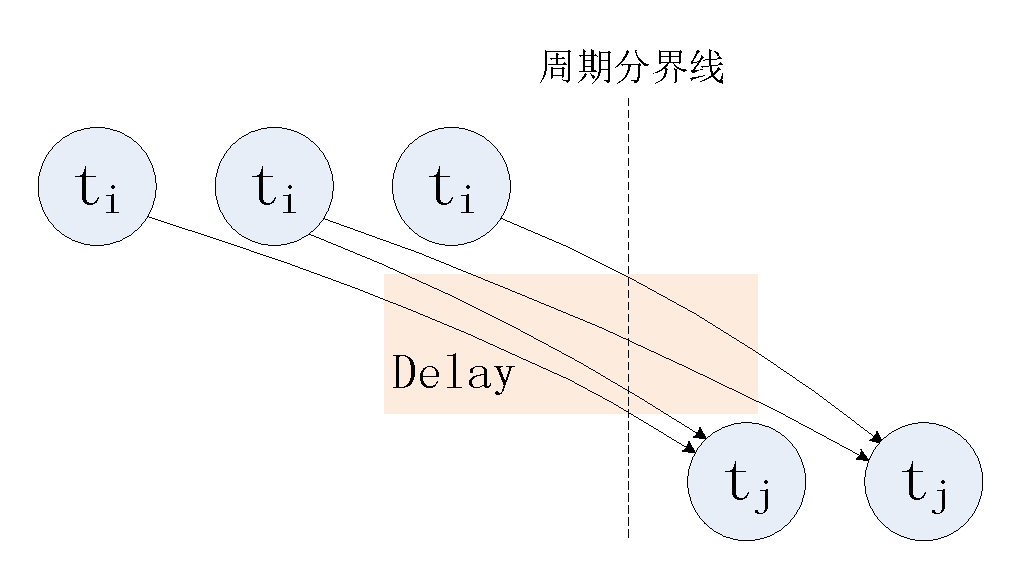
\includegraphics[height=20ex]{figure/DLS-interp.pdf}\\
  \caption{DAG周期间的数据传输关系}\label{DLS-fig-interp}
\end{figure}

明确了这个关系,就容易求得跨周期结点间的数据传输了。继续考察从 $t_i$ 到 $t_j$ 的数据量的对应关系,如图 \ref{DAG-fig-interp-data} 所示。

\begin{figure}[!hbt]
  \centering
  % Requires \usepackage{graphicx}
  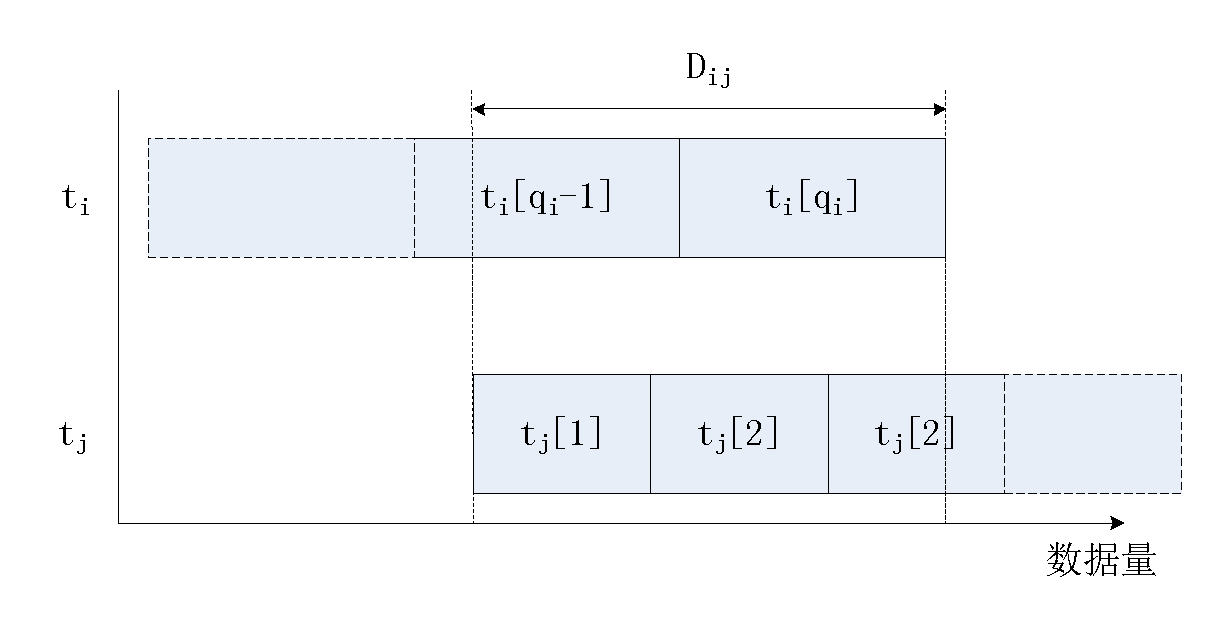
\includegraphics[height=25ex]{figure/DAG-interp-data.pdf}\\
  \caption{DAG中$t_i$与$t_j$周期间的数据对应关系}\label{DAG-fig-interp-data}
\end{figure}

注意到周期内 $t_i$ 的最后 $\left\lceil\frac{D_{ij}}{p_{ij}}\right\rceil$ 个结点发出的最后 $D_{ij}$ 个数据构成了跨周期的 Delay 部分,这些数据根据对应关系将会传给下一周期 $t_j$ 的前 $\left\lceil\frac{D_{ij}}{c_{ij}}\right\rceil$ 个结点。% 补充具体数据对应
与周期内结点间数据的处理方式不同,由于图 \ref{DAG-fig-interp-data} 中 Delay 部分对应数据在 $t_i$ 和 $t_j$ 上没有统一的起止点,无法由单一公式简单描述,只能从一端起逐个考虑 $t_i$ 结点与 $t_j$ 结点之间的数据传输关系。

根据图 \ref{DAG-fig-interp-data} 中 Delay 与 $t_i$ 部分的对应关系,可以求得 $t_i$ 从第
\begin{equation}\label{DAG-eq-interp-solve-w}
  w_i=q_i-\left\lceil\frac{D_{ij}}{p_{ij}}\right\rceil+1
\end{equation}
次运行开始将部分数据作为 Delay 部分传给下一周期的 $t_j$ 结点。该 $t_i$ 结点所要传输的数据大小为
\begin{equation}\label{DAG-eq-interp-solve-r}
  r_{i1}=D_{ij}-(w_i-1)p_{ij}
\end{equation}
而接收数据的 $t_j$ 的第一个结点  $t_j[0]$  需要 $c_{ij}$ 的数据,比较 $r_{i1}$ 与 $c_{ij}$ 的大小,即可知道需要将 $t_i[w_i]$ 结点产生的 $r_{i1}$ 数据部分还是全部传给 $t_j[0]$ 结点。如果 $r_{i1}>c_{ij}$,那么将 $c_{ij}$ 大小的数据传给 $t_j[0]$ 结点,剩余的 $$r_{i2}=r_{i1}-c_{ij}$$ 数据继续向后面的 $t_j$ 结点传送;而如果 $r_{i1}<c_{ij}$,那么 $r_{i1}$ 需要全部传给 $t_j[0]$ 结点,并且还需继续考察后面 $t_i[w_i+1]$ 结点所产生的 $$r_{i2}=p_{ij}$$ 有多少需要传给 $t_j[0]$ 结点……持续以上过程,直到所有 $D_{ij}$ 的数据全部分析完毕,即可求得跨周期的 $t_i$ 与 $t_j$ 结点之间分别有多少数据需要传输。

%下面将以上过程给出较详细的算法描述:
算法 \ref{algo-DAG-interp} 将以上过程给出了较详细的描述。
\begin{algorithm}
  \caption{计算两任务周期间结点间数据传输量}
  \label{algo-DAG-interp}
  \KwIn{GSDF 图}
  \KwOut{DAG 中周期间结点间数据传输量}
  由 \eqref{DAG-eq-interp-solve-w} 和 \eqref{DAG-eq-interp-solve-r} 两式求出 $w_i$ 和 $r_i$\;
  $w_j=0$\;
  $r_j=c_{ij}$\;
  \While{$w_i \leqslant q_i$}{
      \uIf{$r_i < r_j$}{
          trs = $r_i$\;
          添加从 $t_i[w_i]$ 到 $t_j[w_j]$ 结点 trs 大小的数据量\;
          $r_i=p_{ij}$\;
          $w_i=w_i+1$\;
          $r_j=r_j -$ trs\;
      }\Else{
          trs = $r_j$\;
          添加从 $t_i[w_i]$ 到 $t_j[w_j]$ 结点 trs 大小的数据量\;
          $r_j=c_{ij}$\;
          $w_j=w_j+1$\;
          $r_i=r_i -$ trs\;
      }
  }
\end{algorithm}

%\begin{Verbatim}[numbers=left,frame=single,xleftmargin=50pt,commandchars=\\\{\}]
%由以上两式求出 wi 和 ri
%wj = 0
%rj = cij
%WHILE wi <= qi DO
%    IF ri < rj THEN
%        trs = ri
%        添加从 ti[wi] 到 tj[wj] 结点的 trs 大小数据量
%        ri = pij
%        wi = wi + 1
%        rj = rj - trs
%    ELSE
%        trs = rj
%        添加从 ti[wi] 到 tj[wj] 结点的 trs 大小数据量
%        rj = cij
%        wj = wj + 1
%        ri = ri - trs
%    END IF
%END WHILE
%\end{Verbatim}

由以上算法即可容易求得 $t_i$ 到 $t_j$ 结点间跨周期的数据传输量。对 GSDF 内所有 Delay > 0 的结点之间如此进行即可求得所有跨调度周期结点间的数据传输量。

\section{改进的S类算法}
\subsection{算法流程}
结合以上两节周期内与周期间数据传输的不同处理方式,提出改进的S类算法 (ICS 算法)如算法 \ref{algo-ICS} 所述。
\begin{algorithm}
  \caption{Improved Class S (ICS) 算法}
  \label{algo-ICS}
  \KwIn{GSDF 图}
  \KwOut{DAG 中结点间数据传输量}
  求解 GSDF 对应的拓扑矩阵,得到零空间最小整数解向量 $q$\;
  建立初始 DAG 图\;
  向量 $e = 0$\;
  计算初始各边的 buffer 值得到向量 $b$\;
  建立 ready 任务集合 S,根据 $b$ 将满足输入条件的结点加入 S\;
  \While{S 不空}{
      从 S 中取出结点 i\;
      $e_i=e_i+1$\;
      在 DAG 中建立 i 的结点 $t_i[e_i]$\;
      根据 \ref{DAG-innerp} 节算法求出周期内结点间数据通信关系\;
      由 \eqref{basic-eq-SDF} 式更新 $b$\;
      \For{所有根据 $b$ 所得满足输入条件且不在 S 中的结点 $j$}{
          \If{$e_j < q_j$}{
              将结点 $j$ 加入 S\;
          }
      }
  }
  根据 \ref{DAG-interp} 节算法得到所有跨周期结点间数据通信关系\;
\end{algorithm}

%\begin{Verbatim}[numbers=left,frame=single,xleftmargin=50pt,commandchars=\\\{\}]
%求解 GSDF 对应的拓扑矩阵,得到零空间最小整数解向量 q
%建立初始 DAG 图
%向量 e = 0
%计算初始各边的 buffer 值得到向量 b
%建立 ready 任务集合 S,根据 b 将满足输入条件的结点加入 S
%WHILE S 不空 DO
%    从 S 中取出结点 i
%    ei = ei + 1
%    在 DAG 中建立 i 的结点 ti[ei]
%    根据第 2 节算法求出周期内结点间数据通信关系
%    由 2.2 式更新 b
%    FOR 所有根据 b 所得满足输入条件且不在 S 中的结点 j
%        IF ej < qj THEN
%            将结点 j 加入 S
%        END IF
%    END FOR
%END WHILE
%根据第 3 节算法得到所有跨周期结点间数据通信关系
%\end{Verbatim}

以上算法是在 \cite{SDF1987} 所述S类算法基础上改进而成,在将 GSDF 转化为 DAG 的同时还求出了每个运行结点与同其有数据依赖关系的结点之间的通信数据量,包括周期内的和周期之间的通信关系,因此称为改进的S类算法 (Improved Class S, ICS 算法)。

\subsection{复杂度分析}
假设 GSDF 图中顶点数为 $V_G$、边数为 $E_G$,转化出的 DAG 中顶点数为 $V_D$、边数为 $E_D$。
求解 GSDF 拓扑矩阵时,由于矩阵具有特殊性,结点之间是两两产生联系的,因此只用一遍深度优先遍历即可求得最小整数向量,最后再对得到的 $V_G$ 维向量归一化,复杂度为 $O(E_G+V_G)$。计算初始各边 buffer 值需对 GSDF 中各边依次进行,因此复杂度是 $O(E_G)$。

在循环过程中,建立结点的操作一共进行了 $V_D$ 次,复杂度为 $O(V_D)$。
求出周期内与周期间结点间的数据通信关系的过程,将得到 DAG 中所有边上的通信数据量,因此该步的复杂度为 $O(E_D)$。此外,对 GSDF 中每个结点的更新 b 的操作,相当于总的来说对 GSDF 所有边进行一次操作,因此复杂度为 $O(E_G)$。

综上,ICS 算法总的复杂度为 $$O(E_G+V_G)+O(E_G)+O(V_D)+O(E_D)+O(E_G)=O(E_G+V_G+E_D+V_D)$$



\section{本章小结}

本章设计了 COSS 算法的第二步,分析了从 GSDF 转化为 DAG 的方式,以及其过程中所遇到的周期内与周期间的数据传输量计算问题。本章分两节针对以上两个问题分别提出了解决方案,提出了 ICS 算法并详述了算法过程。通过 ICS 算法可以将上一章所得到的 GSDF 转化为对应的包含结点间数据传输量(带权)的DAG,为下一步得到最终的调度表做准备。

